%%
%% Author: lukas
%% 12.02.2019
%%

% Preamble
\documentclass[11pt]{article}

% Packages
\usepackage{amsmath}
\usepackage{graphicx}
\usepackage{amsfonts}



% Document
\begin{document}

    \begin{figure}[ht!]
        \centering
        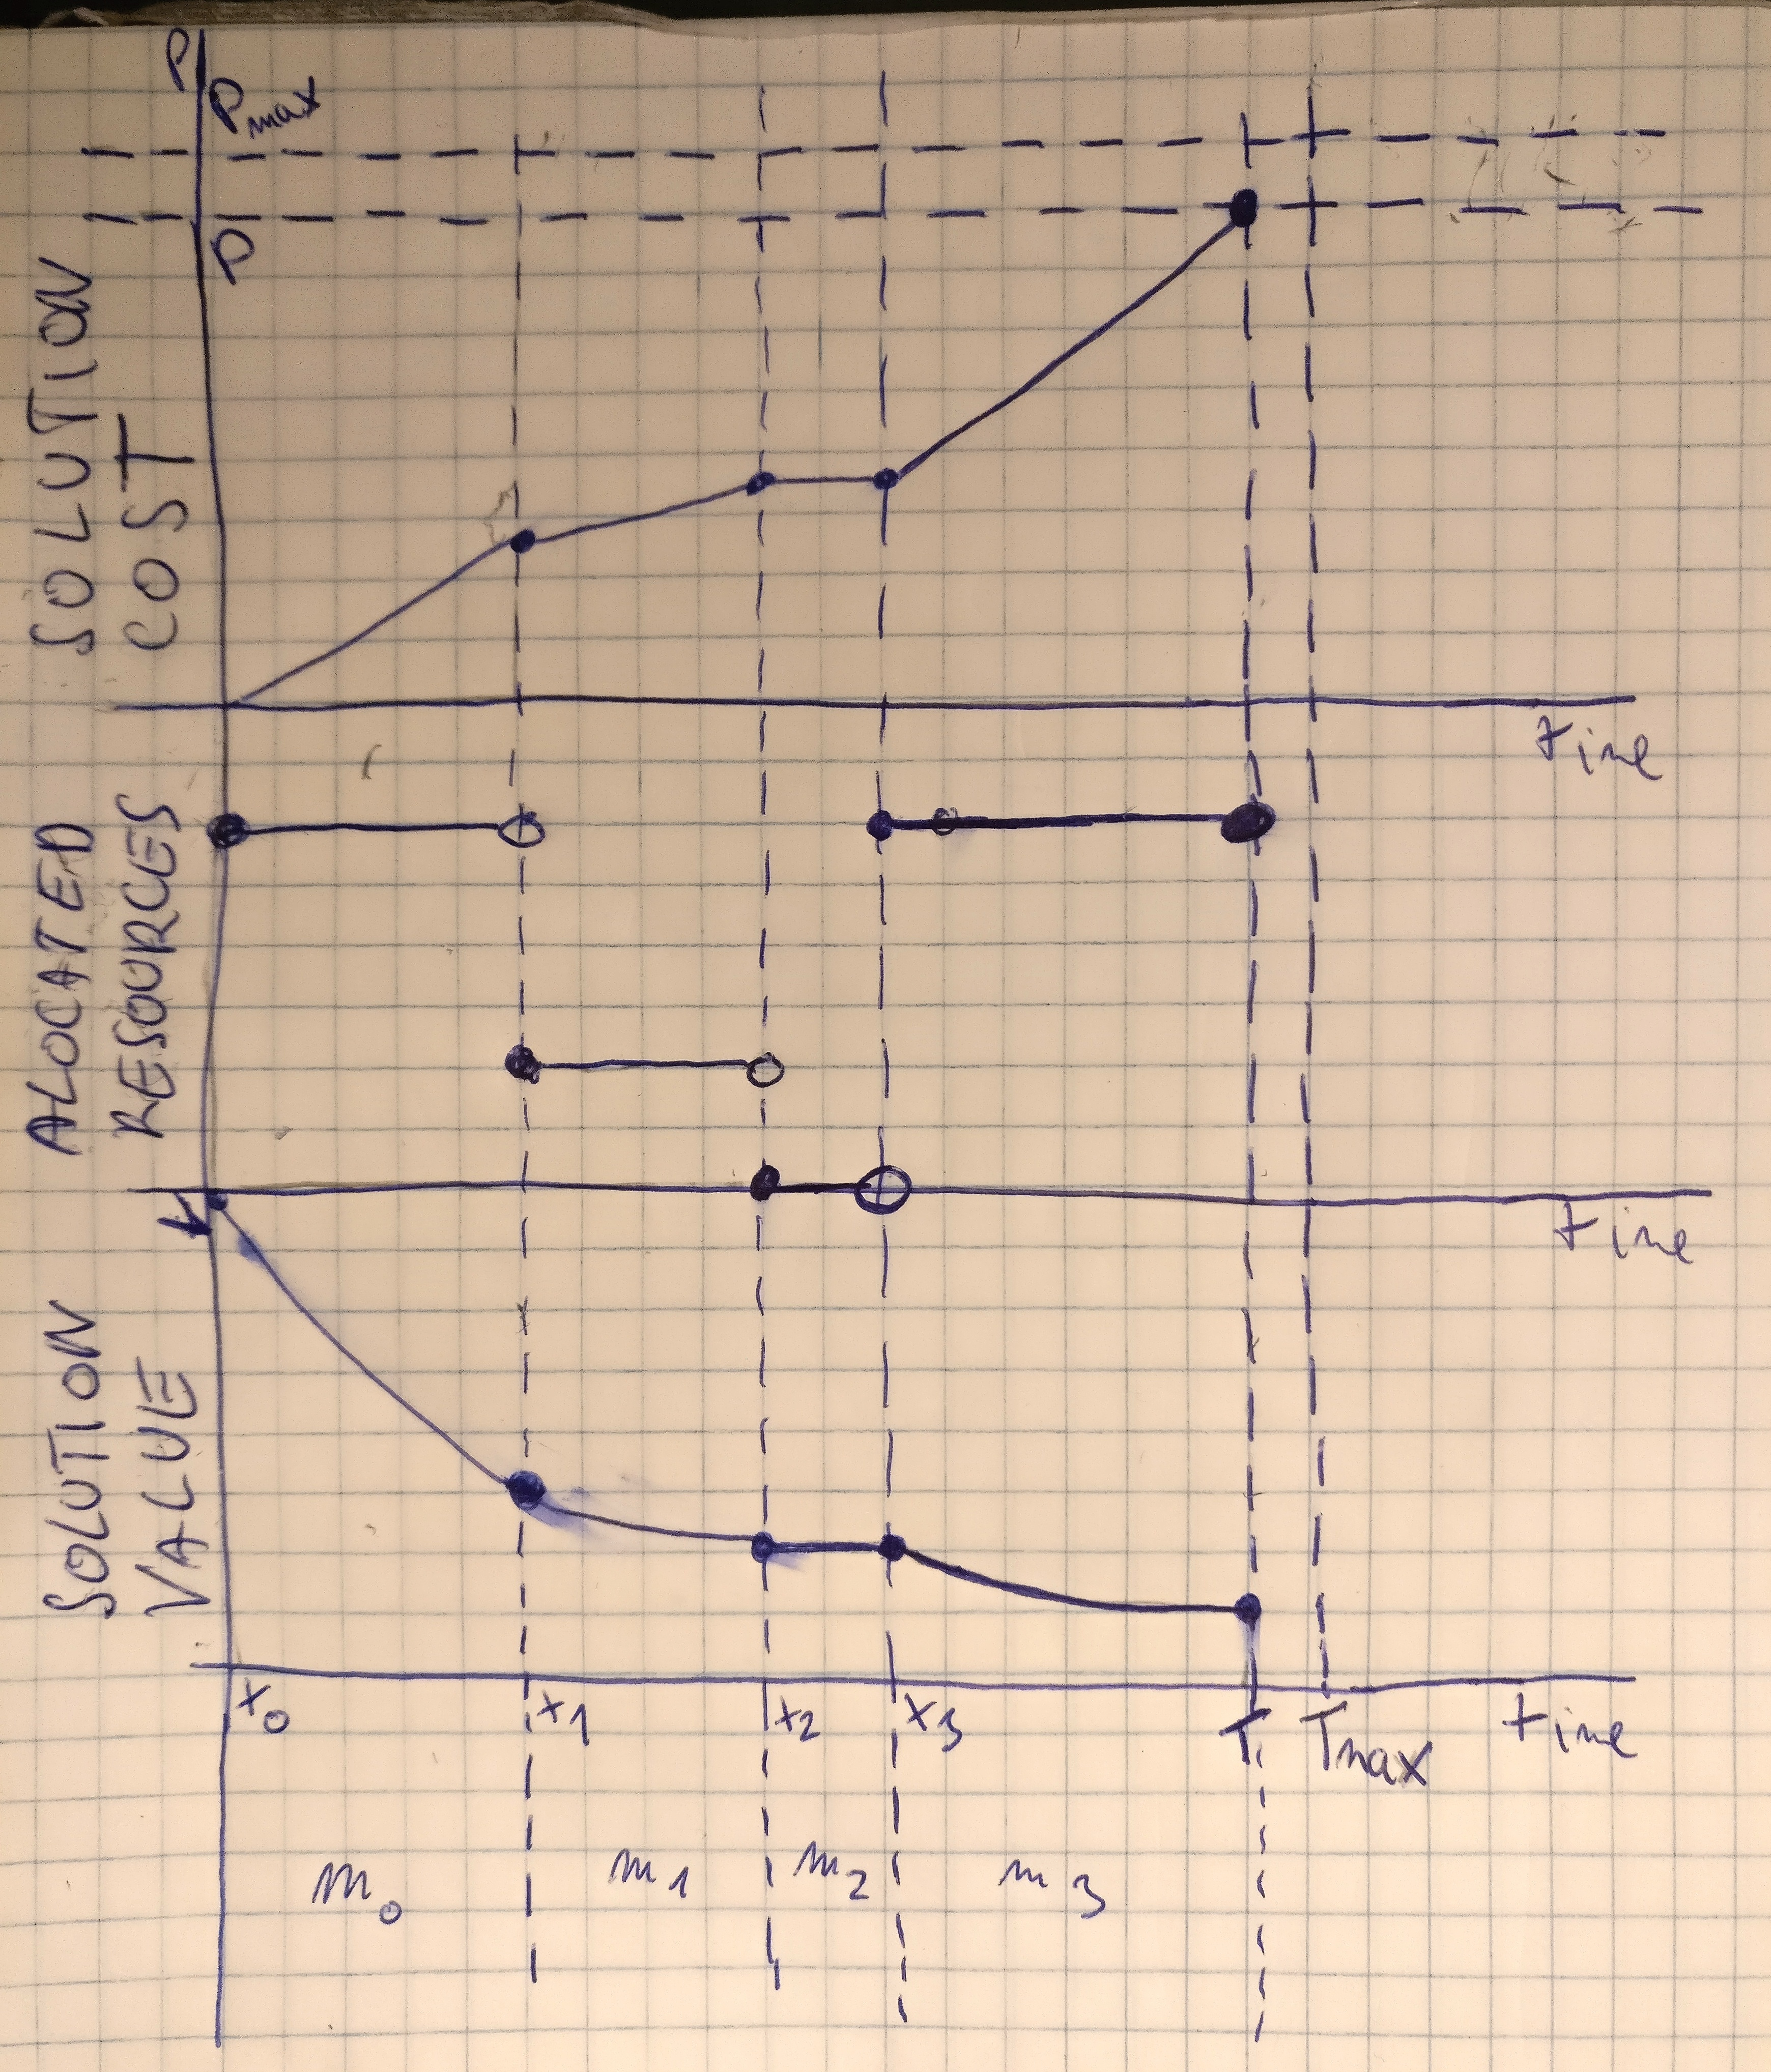
\includegraphics[width=130mm]{table.jpg}
        \caption{grafy ze kterych jsem vychazel}
    \end{figure}

    \newpage

    \begin{itemize}
        \item Horizontální osa reprezentuje čas (tedy jakýkoliv bod na této ose je $t_i$) a je rozdělena na časové intervaly - $m_i$
        \item Vertikální osy jsou následující hodnoty
        \begin{itemize}
            \item \textbf{Solution Cost} - cena za exekuci optimalizačního algoritmu v závislosti na čase - to, kolik se reálně zaplatí za alokované zdroje
            \item \textbf{Allocated resources} - počet alokovaných zdrojů (tedy číslo) v závislosti na čase, dá se dále dělit na CPU, RAM, DISK
            \item \textbf{Solution Value} - cena řešení, které vytvořil optimalizační algoritmus v závislosti na čase
        \end{itemize}
    \end{itemize}

    \section{Moment}\label{sec:m}
    \textbf{M}\ldots\textit{moments} - definují časové intervaly v systému, nový interval začíná vždy ve chvíli, kdy se změnila alokace zdrojů pro určitý job,
    vztahuje se tedy k jobu.
    V podstatě to můžu pojmenovat i jinak, zatím je to pracovní verze.

    Délka časového intervalu je doba, po kterou určitý job měl přidělené určité zdroje a jedná se o časovou hodnotu - tedy například 2 minuty.
    \begin{align*}
        | m_i | = t_{i+1} - t_i
    \end{align*}
    Tedy například v předešlým grafu existují 4 momenty:
    \begin{align*}
        | m_0 | &= t_{1} - 0\\
        | m_1 | &= t_{2} - t_{1}\\
        | m_2 | &= t_{3} - t_{2}\\
        | m_3 | &= T - t_{3}
    \end{align*}

    \section{Solution Value}\label{sec:solution-value}
    \textbf{V}\ldots\textit{solution value} - cena výsledku optimalizačního algoritmu, musí se jednat o fuknci zdrojů a času,
    protože je to závislé - čím více resourců a času, tím je cena výsledného plánu/řešení menší (nicméně tohle nebude lineární závislost)\\
    \subsection{Nápad 1.}\label{subsec:napad-1}
    Obecně to tedy bude vypadat nějak takhle:
    \begin{align*}
        v = f_{a}(t, R, d)
    \end{align*}
    Kde:
    \begin{itemize}
        \item $a$ je algoritmus, který exekuuje daný optimalizační algoritmus (např. TASP) - každý bude mít jinou funkci, protože to řeší jinak
        \item $t$ je délka časového intervalu, při kterém byly dostupné zdroje $R$ (tedy délka momentu, k tomu se dostanu dále)
        \item $d$ jsou daná data, která jsou vstupem algoritmu
    \end{itemize}
    Pak $v = f_{a}$ je definována jako:
    \begin{quotation}
        Schopnost algoritmu $a$ dosáhnout na datech $d$ při alokaci zdrojů $R$ za čas $t$ ceny řešení $v$.
    \end{quotation}
    Pokud tedy použiju \textit{moment} tak je tak hodnota funkce pro každý moment jiná - je závislá na zdrojích, které jsou v každém momentu jiné,
    ale její význam zůstává stejný.
    \begin{align*}
        v_{m_{i}} = f_{a}(|m_{i}|, R_{m_{i}}, d_{m})
    \end{align*}
    Data jsou také závislá na momentu, protože podle definice funke $f_{a}$ musí být data na vstupu do dalšího momentu modifikována tak,
    aby odpovídala částečnému řešení optimalizačního problému z předchozího momentu.

    Jinými slovy, pokud funkce $f_a$ vrátí "plán" na konci momentu $m_i$ musí se tento "plán" vložit do dat pro moment $m_{i+1}$.
    Tedy v každém momentu probíhá zlepšení řešení z předchozího momentu.
    Technicky by to snad mělo být řešitelné (minimálně TASP tohle úmí - můžu mu předhodit částečný plán a on mi ho bude zlepšovat).

    Pak minimální cena celého optimalizační problému (tedy to, co je konečné řešení vráceného uřivateli) se definuje jako:
    \begin{align*}
        v_{j} = \min \{ f_{a}(|m_{j, i}|, R_{j, m_{j, i}}, d_{j, m_{j, i}}) \}
    \end{align*}
    Kde $j$ je id jobu a $i = 0\dots M$, $M$ je počet realokací zdrojů v průběhu času.

    Abych řekl pravdu, tak se mi tady moc nelíbí to $\min$, ale nenapadlo mi, jak bych se toho zbavil

    \subsection{Nápad 2.}\label{subsec:napad-2}
    Druhý pokus o formalizaci funkce pro solution value.\\
    Funkce $f_a$ bude nově iterační a bude reprezentovat zlepšení "nějakého" plánu za jednu iteraci.
    Tedy obecně:
    \begin{align*}
        s = f_a(t, R, d)
    \end{align*}

    \begin{quotation}
        Schopnost algoritmu $a$ zlepšit řešení $d$ při alokaci zdrojů $R$ za čas $t$ na řešení $s$.
    \end{quotation}

    A pokud správně zaindexujeme a použijeme zase \textit{moment} jako měření úseků času:
    \begin{align*}
        s_{j, m_{j,i+1}} &= f_{a}(|m_{j,i}|, R_{j, m_{j, i}}, s_{j, m_{i}})\\
        s_{j, m_{j, 0}} &= \emptyset
    \end{align*}
    Nyní potřebujeme novou funkci, která nám bude říkat hodnotu (solution value) řešení:
    \begin{align*}
        v = h_{a}(s_{j})
    \end{align*}
    Tedy indexované:
    \begin{align*}
        v_{j, m_{j, i}} &= h_{a} ( s_{j, m_{j, i}} )\\
        v_{j, m_{j, i + 1}} & \leq v_{j, m_{j, i}}\\
        v_{j, m_{j, 0}} &= \infty
    \end{align*}
    Ve výsledku tedy budu minimalizovat:
    \begin{align*}
        \min h_{a}(s_{j, m_{j, M}}) = h_{a}(\; f_{a}(|M_{j}|, R_{j, M_{j}}, s_{j, M_{j}-1}) \;)
    \end{align*}
    Kdy vlastně moment $M$ je poslední v časové řadě momentů.\\
    Díky této definici říkám, že ty data (řešení problému) jsou na sobě závislá v čase - nové řešení
    je vždy "dále" v čase.

    \section{Solution Cost}\label{sec:solution-cost}
    Aneb kolik stálo alokování zdrojů - tedy kolik jsem zaplatil např.
    Amazonu za naplánování nějakých dat na CPU/RAM/DISK.\\
    Obecně
    \begin{align*}
        p = g_{h} (t, R)
    \end{align*}
    Kde funkce $g_h$ říká, kolik peněz stojí provozování zdrojů $R$ za čas $t$ u providera zdrojů (ie Amazon) $h$.\\
    Zase bude závislá pro moment a také pro job.
    \begin{align*}
        p_{j, m_{j, i}} = g_{h} (|m_{j,i}|, R_{j, m_{j,i}})
    \end{align*}
    Tedy výsledná cena exekuce jednoho jobu bude:
    \begin{align*}
        p_{j} = \sum_{i = 0}^{M} g_{h} ( |m_{j,i}|, R_{j, m_{j,i}} )
    \end{align*}.

    \section{Závěr}\label{sec:zaver}
    Díky tomu budu schopen vyjádřit solution value a solution cost v každém čase, v jakékoliv konfiguraci alokovaných zdrojů.
    Minimalizuji tedy pro kazdy job $j$:

    \subsection{Napad 1}\label{subsec:napad-11}
    \begin{align*}
        &\min \{\, \min \{ f_{a}(|m_{j, i}|, R_{j, m_{j, i}}, d_{j, m_{j, i}}) \}\, \} \qquad \text{for } i = 0\dots M \\
        &\min \sum_{i = 0}^{M} g_{h} ( |m_{j,i}|, R_{j, m_{j,i}} )
    \end{align*}

    \subsection{Napad 2}\label{subsec:napad-22}
    \begin{align*}
        &\min h_{a}(s_{j, m_{j, M}})\\
        &\min \sum_{i = 0}^{M} g_{h} ( |m_{j,i}|, R_{j, m_{j,i}} )
    \end{align*}
    Tedy v tomto pripade hledam idealni koncový moment $M$ a řadu konfigurací $R$ takovou, aby výsledek
    byl co nejmenší.
\end{document}